\makeatletter\let\ifGm@compatii\relax\makeatother
% Problemas con el paquete geometry se solucionan con la anterior
% sentencia. 18/5/2015
\documentclass[10pt]{beamer}

\usetheme{Warsaw}

\usecolortheme{beaver}

%\usepackage[utf8]{inputenc}
\usepackage[latin1]{inputenc}
\usepackage[spanish]{babel}

\usepackage{graphicx}
\usepackage{epstopdf}
\usepackage{multicol}
\usepackage{multirow}
\usepackage{hyperref}
\usepackage{url}
\usepackage{multicol}

\usepackage{appendix}
\usepackage{pdflscape}	%rotacion 90º paginas y las muestra rotadas
\usepackage[square]{natbib}
\usepackage{rotating}




\epstopdfDeclareGraphicsRule{.gif}{png}{.png}{%
  convert gif:#1 png:\OutputFile
}
\AppendGraphicsExtensions{.gif}


\newcommand{\gt}{>}

%-----------------Titulo y autores

\title{Cap\'itulo 1 \\
	Paneles de Instrumentos}
\subtitle{Instrumentos y Avi\'onica}
\author{ Ing. Jorge Garcia}
\institute{
	
\includegraphics[height=1.5cm]{imagenes/logos/400-anios} \hspace{3mm}	
	
\includegraphics[height=1cm]{imagenes/logos/logoUNC} \hspace{1mm}	
	
\includegraphics[height=1cm]{imagenes/logos/fcefyn} \hspace{1mm}	
	
\includegraphics[height=1cm]{imagenes/logos/dpto-aero-logo}
	\\
%	Departamento de Aeron\'autica \\
%	Facultad de Ciencias Exactas, F\'isicas y Naturales \\
%	Universidad Nacional de C\'ordoba
	}
\date{A\~no 2016}


%----------------------------------CONTENIDO------------------

% Capítulo 1. Paneles de Instrumentos
% 1.1. Introducción al estudio del instrumental.
% 1.2. Clasificación de los Instrumentos.
% 1.3. Distribución Normalizada del Instrumental en el Tablero
% 1.4. Presentación en Pantalla Electrónica.

\begin{document}

%----------- titlepage -----------%
\begin{frame}[plain]
  \titlepage
\end{frame}

% \addtobeamertemplate{frametitle}{}{%
% 	\begin{tikzpicture}[remember picture,overlay]
% 	\node[anchor=north east,yshift=4pt] at (current page.north east) 
% 	{\includegraphics[height=0.65cm]{400-anio}\hspace{1.5mm}
% 	
\includegraphics[height=0.5cm]{logo}\hspace{1mm}	
%  	
\includegraphics[height=0.5cm]{logo_fcefyn_cuadrado_solo} \hspace{1mm}	
%  	
\includegraphics[height=0.5cm]{dpto-aero-logo}
% 	};
%	\end{tikzpicture}
% 	\begin{textblock*}{190mm}(.85\textwidth,-1cm)
% 	\includegraphics[height=0.75cm]{400-anio}\hspace{1mm}	
% 	
\includegraphics[height=0.5cm]{logo} \hspace{1mm}	
% 	
\includegraphics[height=0.5cm]{logo_fcefyn_cuadrado_solo.jpg} \hspace{1mm}	
% 	
\includegraphics[height=0.5cm]{dpto-aero-logo.jpg}
% \end{textblock*}}	
%}

\section{Paneles de instrumentos}
\label{sec:paneles.instrumentos}

\begin{frame}{Paneles de instrumentos}

\tableofcontents[pausesections]
  
\end{frame}


% \AtBeginSubsection[]
% {
% \begin{frame}{Introducci\'on al estudio del instrumental}
% \tableofcontents[currentsection,currentsubsection]
% \end{frame}
% }

\subsection{Introducci\'on al estudio del instrumental}
\label{sec:cap.1.1.introduccion.estudio.instrumental}

\begin{frame}{Introducci\'on al estudio del instrumental}
  
  \begin{tabular}{ccc}
    {\bf \large 1903} & & {\bf \large 2005} \\ & & \\
	{Wright Flyer I} & & {Airbus A380} \\ & & \\
    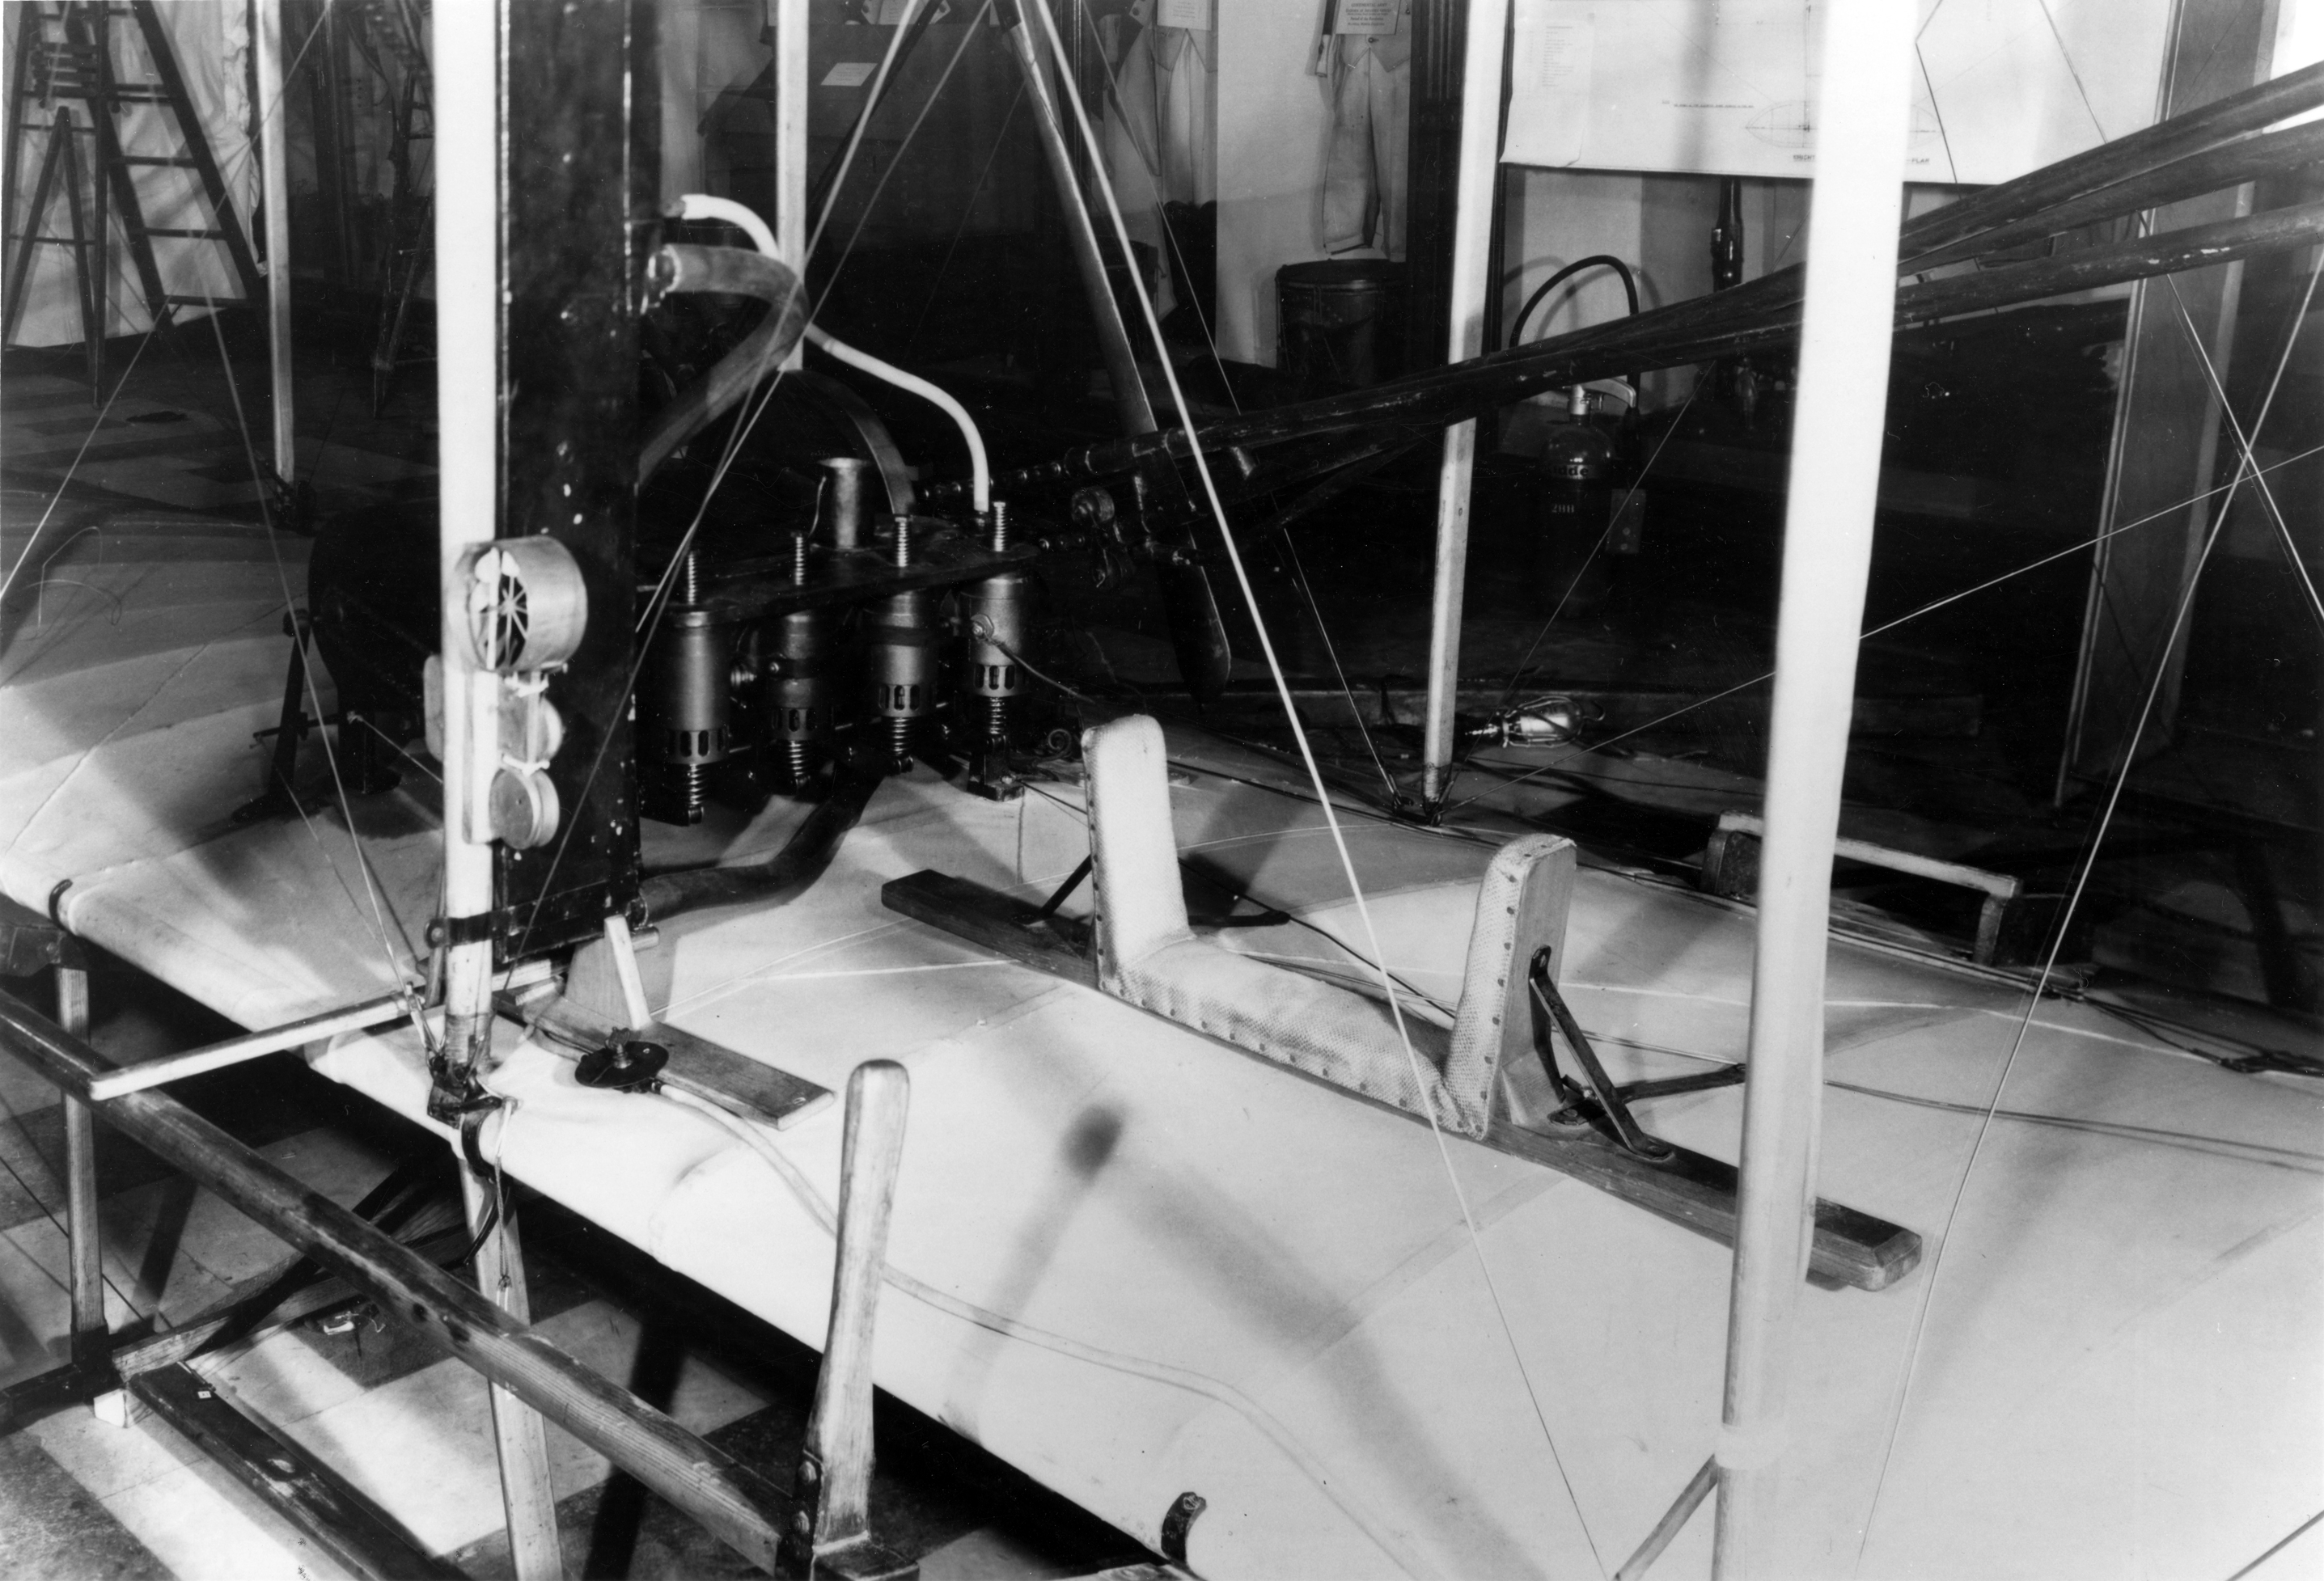
\includegraphics[width=0.45\textwidth]{imagenes/1.1.introduccion/wright_brothers_instruments.jpg}
	& \hspace{5mm}
	&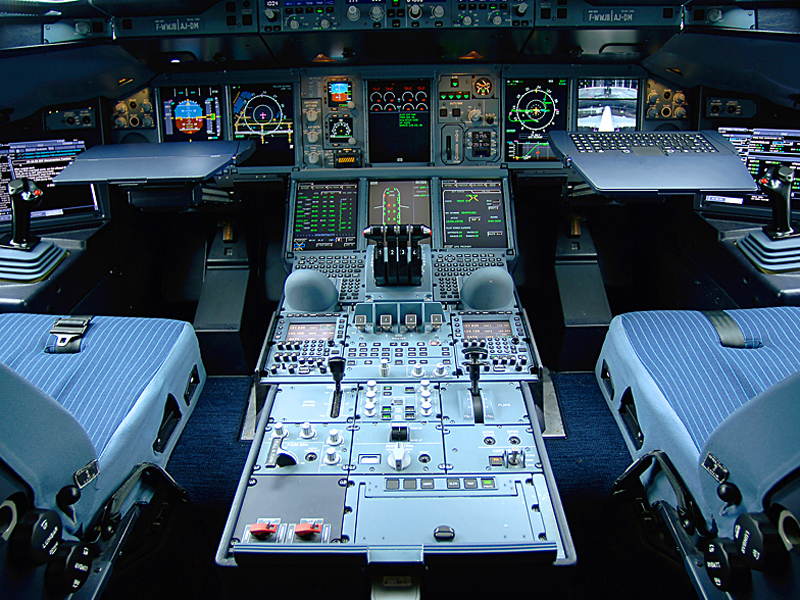
\includegraphics[width=0.45\textwidth]{imagenes/1.1.introduccion/A380_Cockpit_2.jpg} \\ & & \\
\parbox{0.4\textwidth}{\small
	Tres (3) instrumentos: \\
	\mbox{cron\'ometro}, anem\'ometro,\\ tac\'ometro}
	& & ¡Muchos instrumentos! \\
  \end{tabular}

\end{frame}

\begin{frame}{Introducci\'on al estudio del instrumental}

 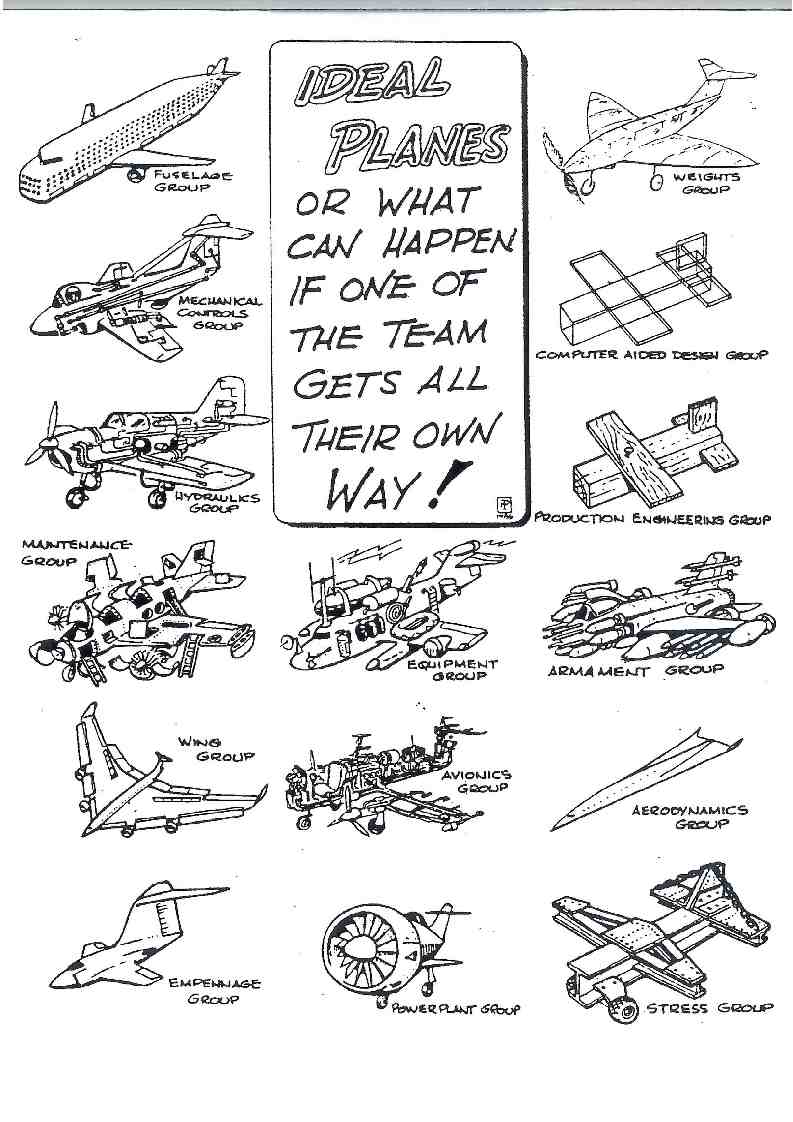
\includegraphics[width=0.5\linewidth]{imagenes/1.1.introduccion/IntelligentDesignMain}

\end{frame}

\begin{frame}{Introducci\'on al estudio del instrumental}

  \begin{block}{Instrumentos de vuelo}
    Instrumentos que se utilizan para mostrar informaci\'on de la
    aeronave y controlar la orientaci\'on de la misma durante el vuelo
  \end{block}

  \begin{columns}{2}

    \begin{column}{0.5\textwidth}
{\small
  \begin{block}{    Necesidades a cumplir:}
    \begin{itemize}
    \item Permitir volar en condiciones de clim\'aticas desfavorables, 
	con escasa visibilidad y durante la noche
    \item Asegurar una operaci\'on segura y confiable
    \item Dar avisos tempranos sobre cualquier falla en los sistemas
      de la aeronave o partes de la misma, de forma que los pilotos
      puedan tomar una acci\'on inmediata
    \end{itemize}
  \end{block}
}
\end{column}
    \begin{column}{0.5\textwidth}
 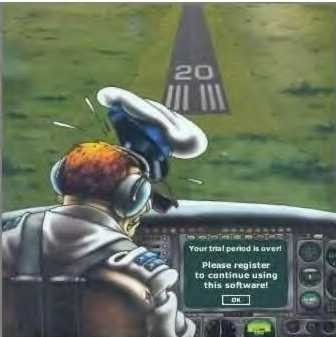
\includegraphics[width=\linewidth]{imagenes/1.1.introduccion/problema_soft.jpg} \\
    \end{column}
  \end{columns}

\end{frame}

\subsection{Clasificaci\'on de los Instrumentos}
\label{sec:cap.1.2.clasificacion.instrumentos}

\begin{frame}{Clasificaci\'on de los Instrumentos}

  \begin{columns}
    \begin{column}{0.5\textwidth}
      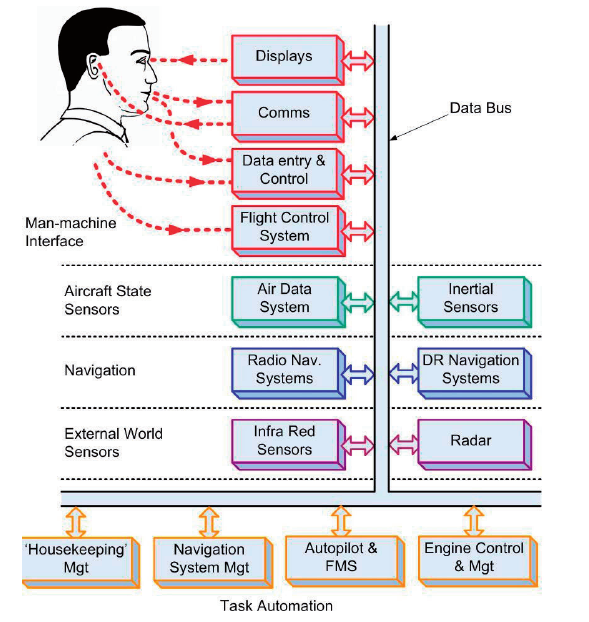
\includegraphics[width=\linewidth]{imagenes/1.2.clasificacion.instrumentos/tipos_instrumentos.png}

      {\tiny Referencia: Collinson, {\it Introduction to Avionics
          Systems}, 2011 }
    \end{column}
  \begin{column}{0.5\textwidth}
    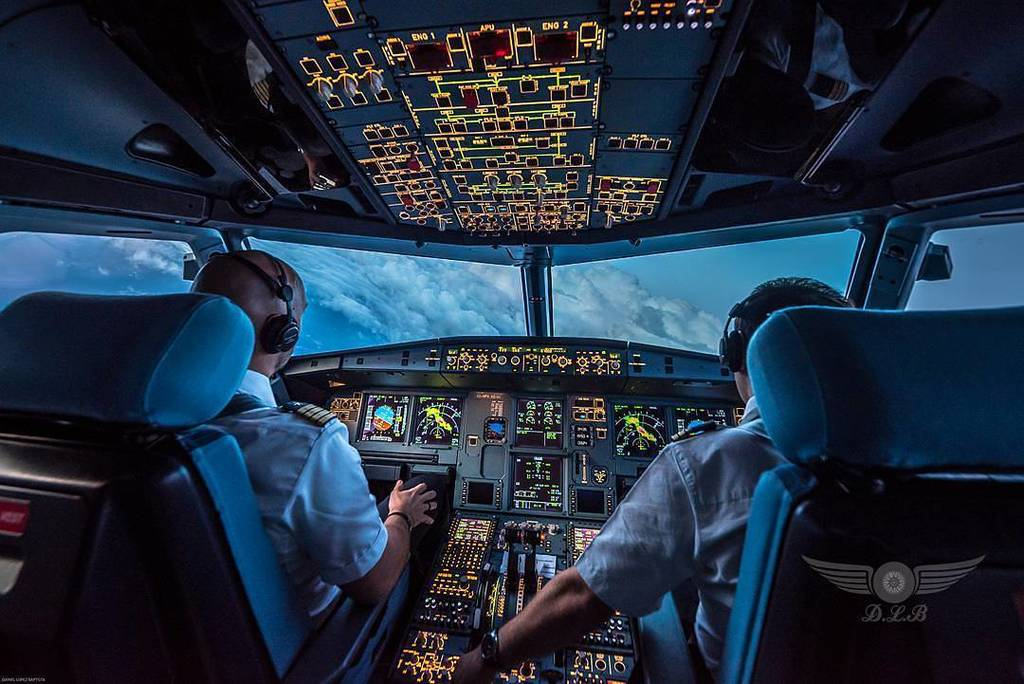
\includegraphics[width=\linewidth]{imagenes/1.2.clasificacion.instrumentos/glass_cockpit.jpg}
%    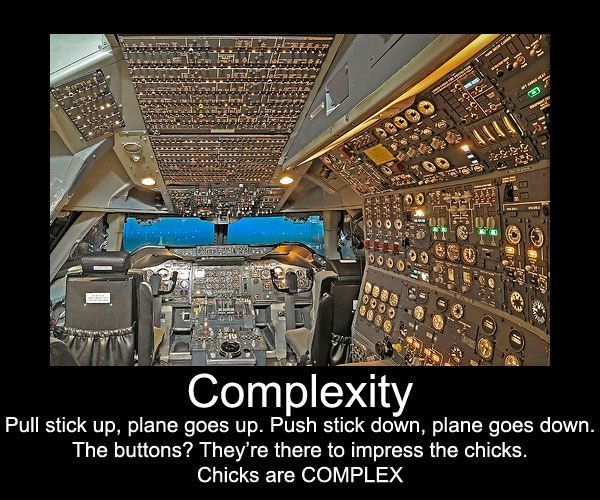
\includegraphics[width=\linewidth]{imagenes/1.2.clasificacion.instrumentos/humor_complejidad.jpg}
  \end{column}
  \end{columns}

\end{frame}

\begin{frame}{Clasificaci\'on de los Instrumentos}

  \begin{itemize}
  \item {\bf Instrumentos del sistema pitot-est\'atica}
  \item {\bf Instrumentos girosc\'opicos}
  \item {\bf Instrumentos duplicados}
  \item {\bf Instrumentos de navegaci\'on}
  \item {\bf Instrumentos del grupo motopropulsor}
  \end{itemize}

\end{frame}

\begin{frame}{Clasificaci\'on de los Instrumentos}

  \begin{itemize}
  \item {\bf Presentaciones cuantitativas}
    \begin{itemize}
      \item Escala circular
      % \begin{itemize}
      %    \item Escala lineal
      %    \item Escala no lineal (cuadr\'atica, logar\'itmica}
      % \end{itemize}
       \item Escala longitudinal
    \end{itemize}
  \item {\bf Presentaciones cualitativas}
  \item {\bf Presentaciones directoras}
  \end{itemize}

\end{frame}

\begin{frame}{Clasificaci\'on de los Instrumentos}

  \begin{tabular}{ccc}
    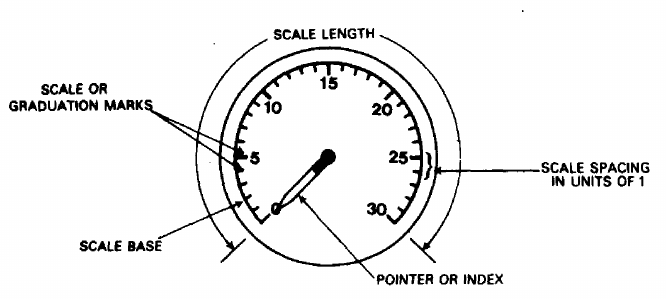
\includegraphics[width=0.45\textwidth]{imagenes/1.2.clasificacion.instrumentos/escala_circular_cuantitativa.png} & \hspace{3mm}
&     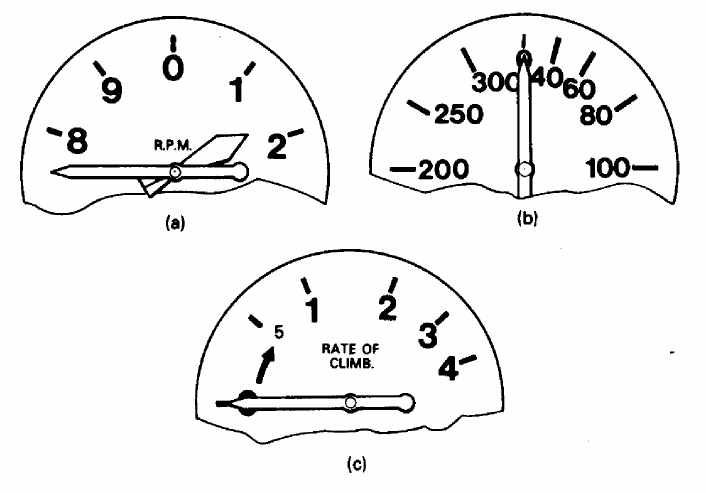
\includegraphics[width=0.45\textwidth]{imagenes/1.2.clasificacion.instrumentos/escala_circular_lineal_no_lineal.png}
\\
	Escala circular cuantitativa & 
& \parbox{0.45\textwidth}{a) Lineal, b) ley cuadr\'atica, \\c) ley logaritmica}
\\
  \end{tabular}

\end{frame}

\begin{frame}{Clasificaci\'on de los Instrumentos}

  \begin{tabular}{ccc}
    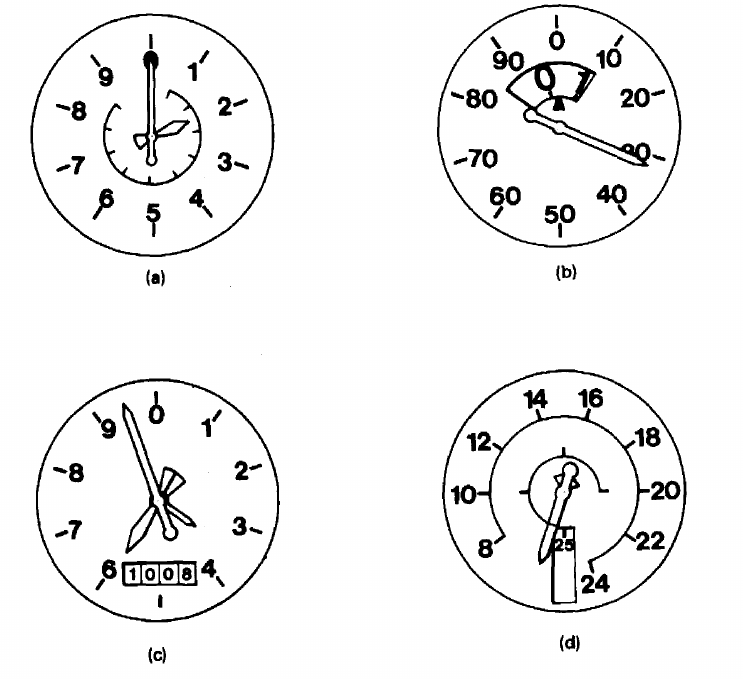
\includegraphics[width=0.45\textwidth]{imagenes/1.2.clasificacion.instrumentos/escala_gran_alcance.png} & \hspace{3mm}
&     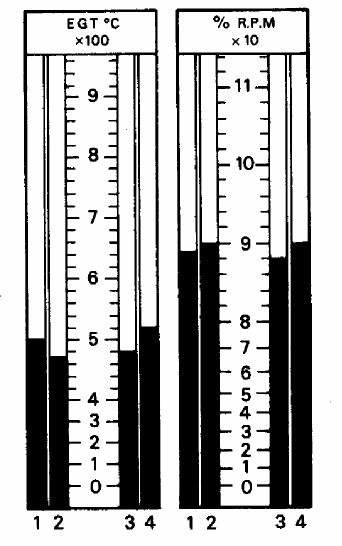
\includegraphics[width=0.35\textwidth]{imagenes/1.2.clasificacion.instrumentos/longitudinal.png}
\\
\parbox{0.45\textwidth}{a)Escalas conc\'entricas, (b) escalas fijas y giratorias, (c) escala com\'un tres agujas, (d) aguja dividida}
&
& Escala longitudinal
\\
  \end{tabular}

\end{frame}

\begin{frame}{Clasificaci\'on de los Instrumentos}

  \begin{tabular}{ccc}
    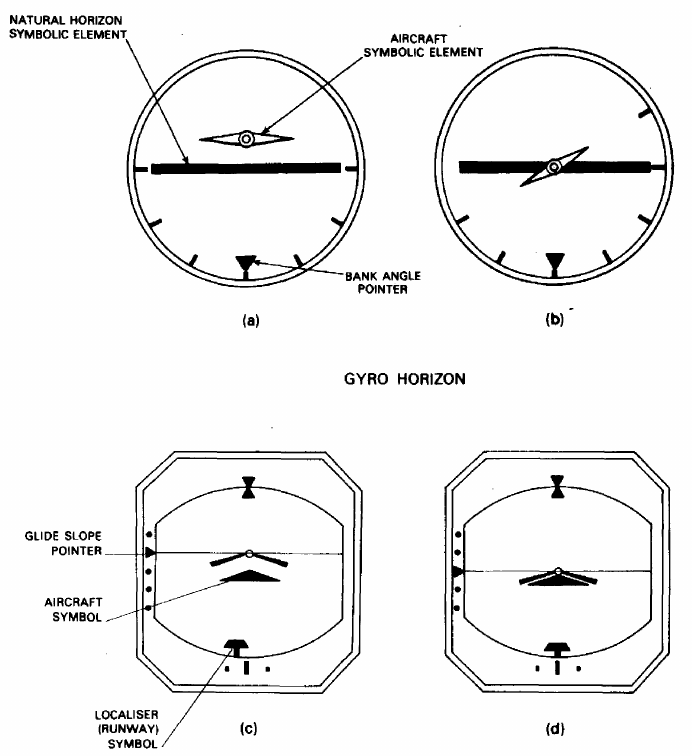
\includegraphics[width=0.45\textwidth]{imagenes/1.2.clasificacion.instrumentos/director.png} & \hspace{3mm}
&     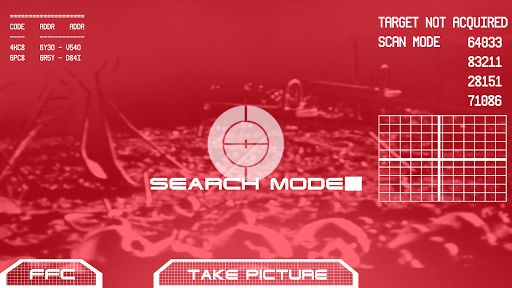
\includegraphics[width=0.5\textwidth]{imagenes/1.2.clasificacion.instrumentos/terminator_hud.png}
\\
\parbox{0.45\textwidth}{Director de vuelo}
&
& Terminator Hud
\\
  \end{tabular}

\end{frame}

\begin{frame}{Clasificaci\'on de los Instrumentos}

{
\includegraphics[width=0.1\textwidth]{imagenes/Video.png}}\,
The Evolution of the Head-Up Display \url{https://www.youtube.com/watch?v=ypIbmfm7n8A}
\vspace{3mm}

  \begin{tabular}{ccc}
    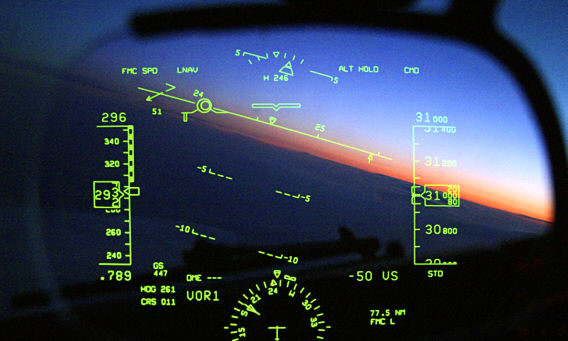
\includegraphics[width=0.45\textwidth]{imagenes/1.2.clasificacion.instrumentos/hud.jpg} & \hspace{3mm}
&     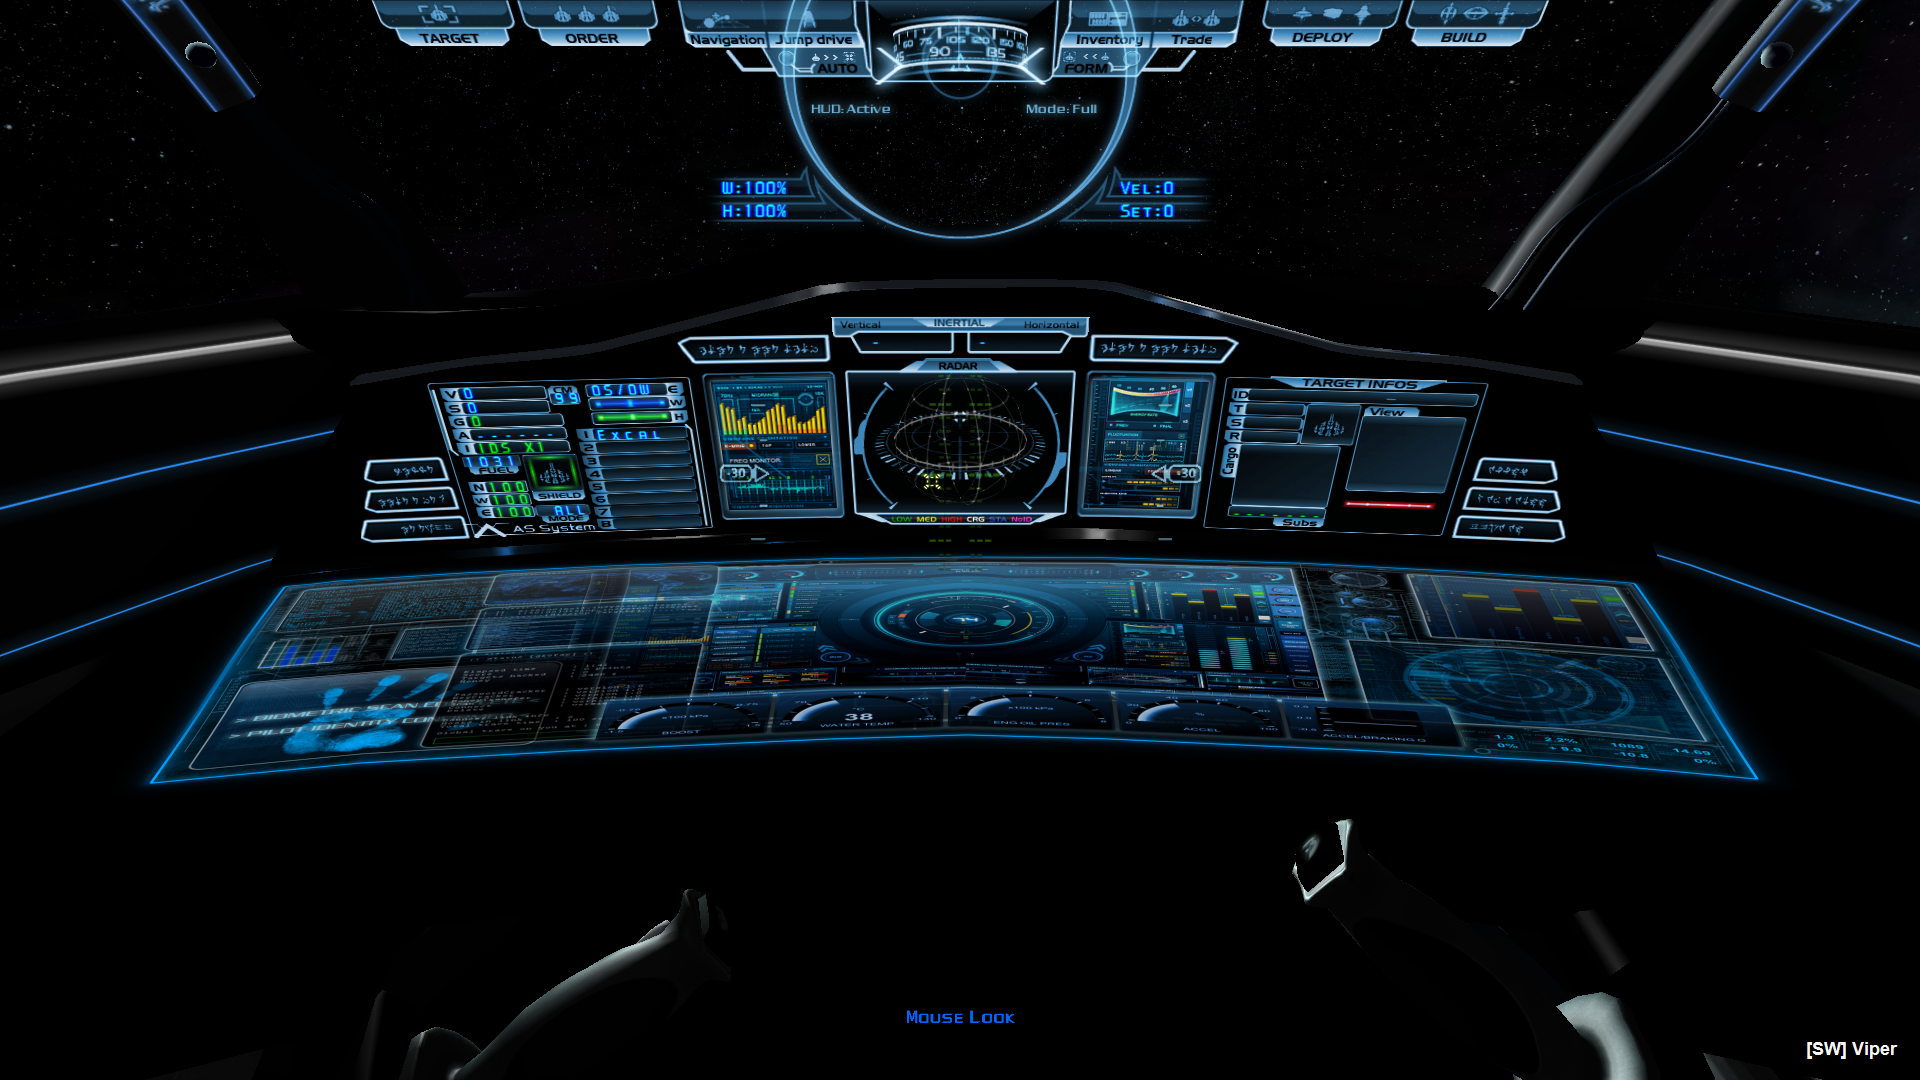
\includegraphics[width=0.5\textwidth]{imagenes/1.2.clasificacion.instrumentos/viper_11.png}
\\
\parbox{0.45\textwidth}{Head Up Display}
&
& Hud futuro
\\
  \end{tabular}

\end{frame}

\begin{frame}{Clasificaci\'on de los Instrumentos}



\vspace{3mm}

{
\includegraphics[width=0.1\textwidth]{imagenes/Video.png}}\,
Enhanced Flight Vision System \url{https://www.youtube.com/watch?v=DR9lyAM2YNE}

\vspace{3mm}

  \begin{tabular}{ccc}
    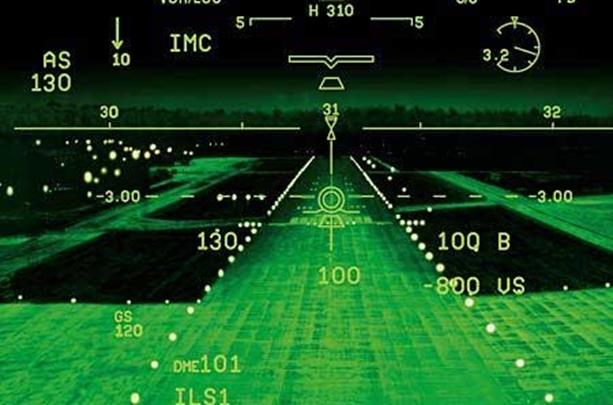
\includegraphics[width=0.45\textwidth]{imagenes/1.2.clasificacion.instrumentos/EFVS_Photo.jpg} & \hspace{3mm}
    &     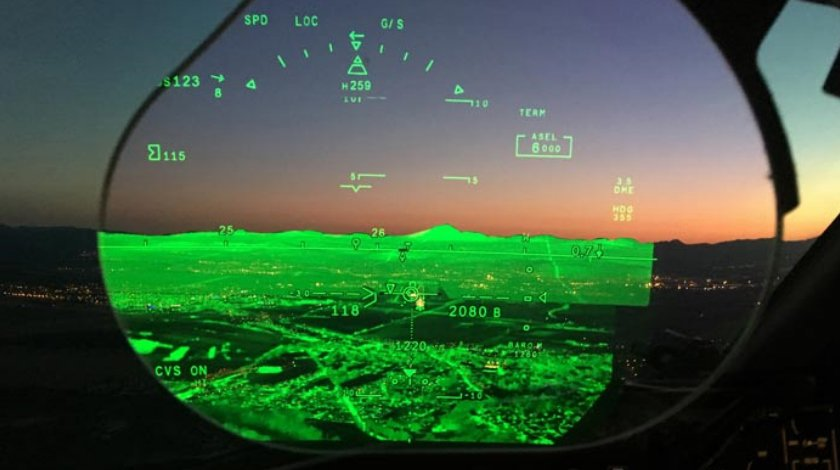
\includegraphics[width=0.45\textwidth]{imagenes/1.2.clasificacion.instrumentos/efvs.jpg} \\
  \end{tabular}
  

\end{frame}



\begin{frame}{Clasificaci\'on de los Instrumentos}

{\Large \bf Avi\'onica = Aviaci\'on + Electr\'onica}

\end{frame}


\subsection{Distribuci\'on Normalizada del Instrumental en el Tablero}
\label{sec:distribucion.normalizada.instrumental.en.el.tablero}

\begin{frame}{Distribuci\'on Normalizada del Instrumental en el
 Tablero}
  

REGULACIONES ARGENTINAS DE AVIACI\'ON CIVIL (RAAC)\\
PARTE 91 - REGLAS DE VUELO Y OPERACI\'ON GENERAL\\
SUBPARTE C - REQUERIMIENTOS DE EQUIPAMIENTOS, INSTRUMENTOS Y DE
CERTIFICADOS\\

\vspace{3mm}

\colorbox{yellow!30}{\parbox{0.9\textwidth}{{\bf 91.205} \qquad
Requerimientos de instrumentos y equipamiento para aeronaves civiles motorizadas con
Certificado de Aeronavegabilidad Est\'andar de la Rep\'ublica Argentina}
}

\href{run:biblio/parte-91-19feb2016-res-77-16.pdf}{
\includegraphics[width=0.1\textwidth]{imagenes/libro.png}}
\hspace{3mm}
\href{http://www.anac.gov.ar/anac/web/uploads/normativa/raac/raac_vigentes/por_parte/parte-91-23dic2014.pdf}{
\includegraphics[width=0.15\textwidth]{imagenes/www-logo.png}}

\end{frame}

\begin{frame}{Distribuci\'on Normalizada del Instrumental en el
 Tablero}

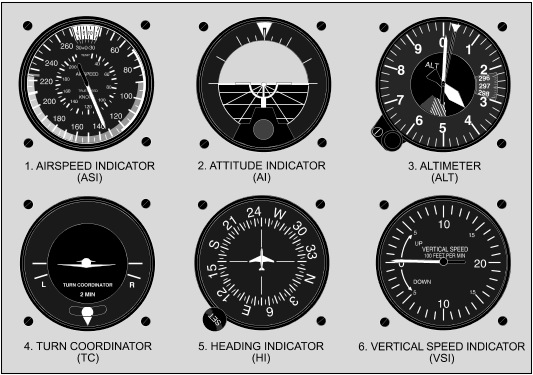
\includegraphics[width=0.9\textwidth]{imagenes/1.3.distribucion.normalizada.instrumental.en.tablero/6_pack.png}

\end{frame}

\begin{frame}{Distribuci\'on Normalizada del Instrumental en el
 Tablero}
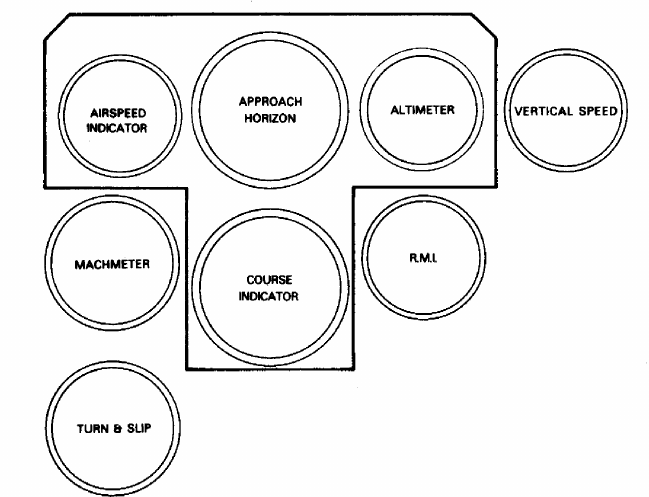
\includegraphics[width=0.9\textwidth]{imagenes/1.3.distribucion.normalizada.instrumental.en.tablero/6.png}

\end{frame}

\begin{frame}{Distribuci\'on Normalizada del Instrumental en el
 Tablero}
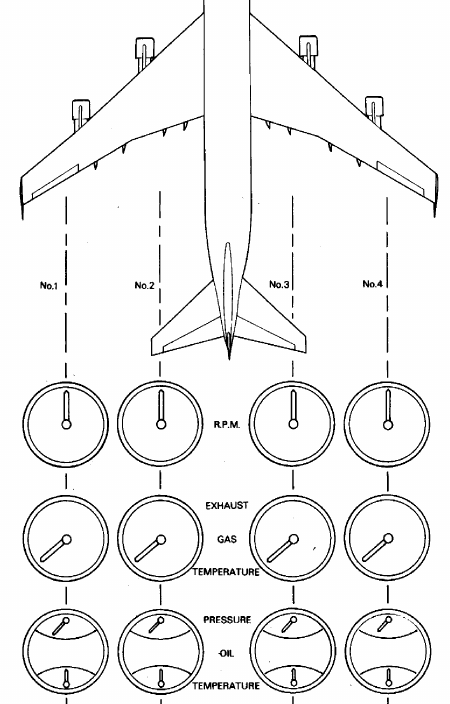
\includegraphics[width=0.4\textwidth]{imagenes/1.3.distribucion.normalizada.instrumental.en.tablero/instrumentos_motor.png}
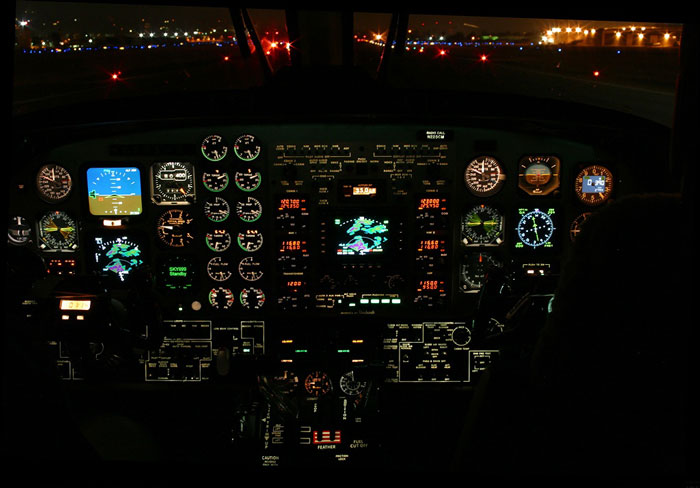
\includegraphics[width=0.6\textwidth]{imagenes/1.3.distribucion.normalizada.instrumental.en.tablero/iluminacion.jpg}

\end{frame}

\subsection{Presentaci\'on en Pantalla Electr\'onica}
\label{sec:cap.1.4.presentacion.en.pantalla.electronica}

\begin{frame}{Presentaci\'on en Pantalla Electr\'onica}

 \begin{block}{Un poco de historia}

     \begin{tabular}{ccl}
     1970& &\parbox{0.75\linewidth}{NASA investigaci\'on en como mostrar instrumentos de vuelo}\\
	& & \\
     1982& &Boeing 767 con pantallas electr\'onicas de datos \\
	& & \\
     1990&& \parbox{0.75\linewidth}{Fines de la d\'ecada, pantallas LCD reemplazan pantallas CRT} \\
	& & \\
     Actualidad&& \parbox{0.75\linewidth}{La mayor\'ia de las aeronaves equipadas con pantallas LCD} \\
   \end{tabular}
 \end{block}
\end{frame}

\begin{frame}{Presentaci\'on en Pantalla Electr\'onica}

  \begin{block}{ EIS (Electronic Instrument
      System)}

Ejemplos:

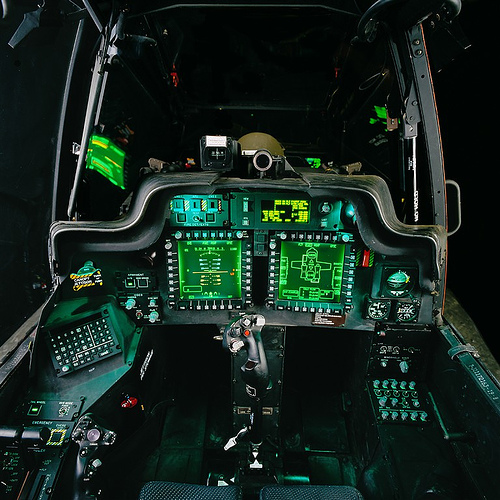
\includegraphics[width=0.34\textwidth]{imagenes/1.4.pantalla.electronica/apache.jpg}
\hspace{3mm}
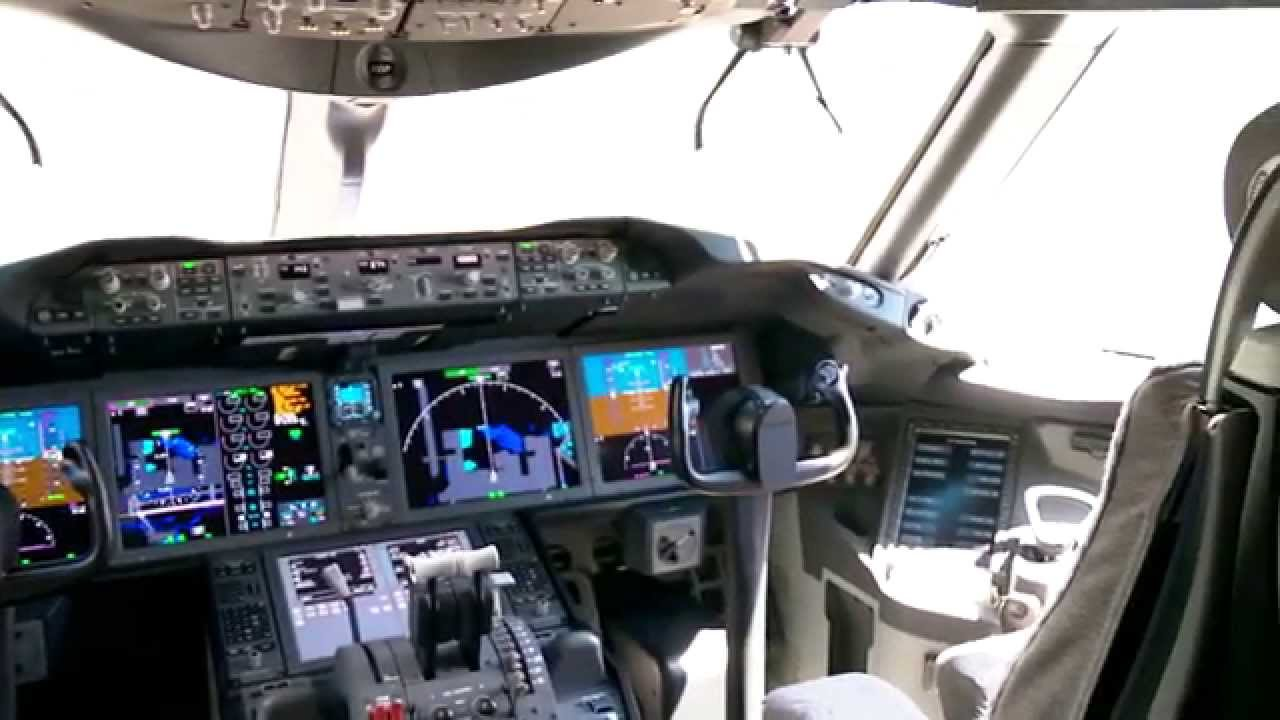
\includegraphics[width=0.55\textwidth]{imagenes/1.4.pantalla.electronica/dreamliner.jpg}

Helic\'optero Apache \hspace{25mm} Boeing 787 Dreamliner
  \end{block}

\end{frame}

\begin{frame}{Presentaci\'on en Pantalla Electr\'onica}
  Una instalaci\'on EIS sigue la secuencia siguiente:

\vspace{3mm}


 Pantallas \qquad $\Longrightarrow$ \qquad
 Controles  \qquad $\Longrightarrow$ \qquad
 Procesadores de datos 


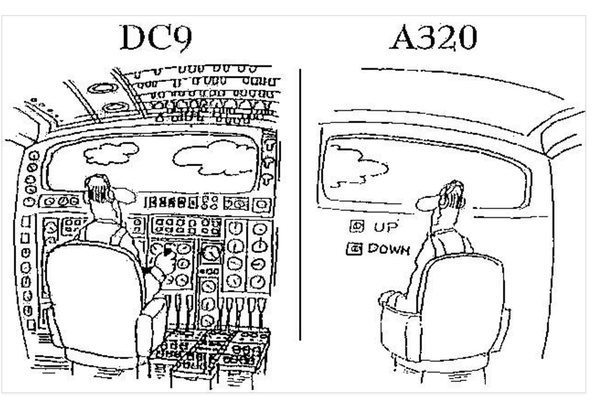
\includegraphics[width=0.85\textwidth]{imagenes/1.4.pantalla.electronica/efis_humor.png}


\end{frame}

\begin{frame}{Presentaci\'on en Pantalla Electr\'onica}

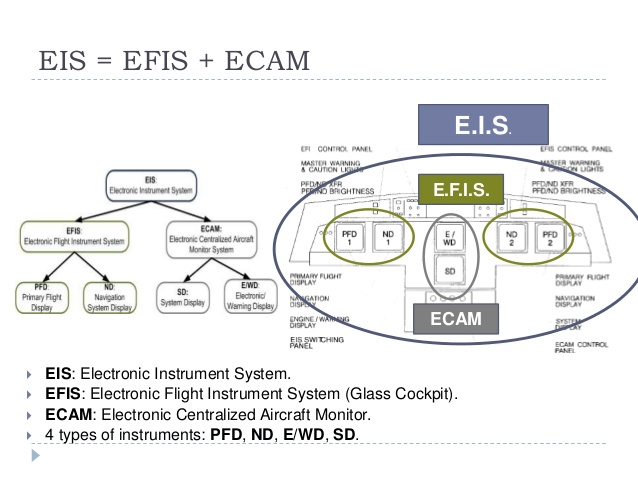
\includegraphics[width=0.85\textwidth]{imagenes/1.4.pantalla.electronica/efis.jpg}

\end{frame}

\begin{frame}{Presentaci\'on en Pantalla Electr\'onica}

     \begin{block}{ PFD: Primary Flight Display}
{\footnotesize
	% Presenta los siguientes instrumentos
	
	%  Airspeed Indicator, 
	%  Altimeter, 
	%  HSI (Horizontal Situation Indicator),
	%  VSI (Vertical Speed Indicator)
	

	El PFD reemplaza a los seis (6) instrumentos tradicionales

	Muestra la informaci\'on cr\'itica de vuelo 
	incluyendo velocidad, altitud,direcci\'on (heading)
	actitud y velocidad vertical

	Est\'a dise\~nado para mejorar las alertas al piloto
	al integrar informaci\'on en una sola pantalla

	Reduce el tiempo para monitorear otros instrumentos

	Alerta a los pilotos de condiciones potencialmente peligrosas
        cambiando el color o la forma en el display o mediante alertas
        de sonido. (baja velocidad, alta tasa de descenso) 
}
    \end{block}

 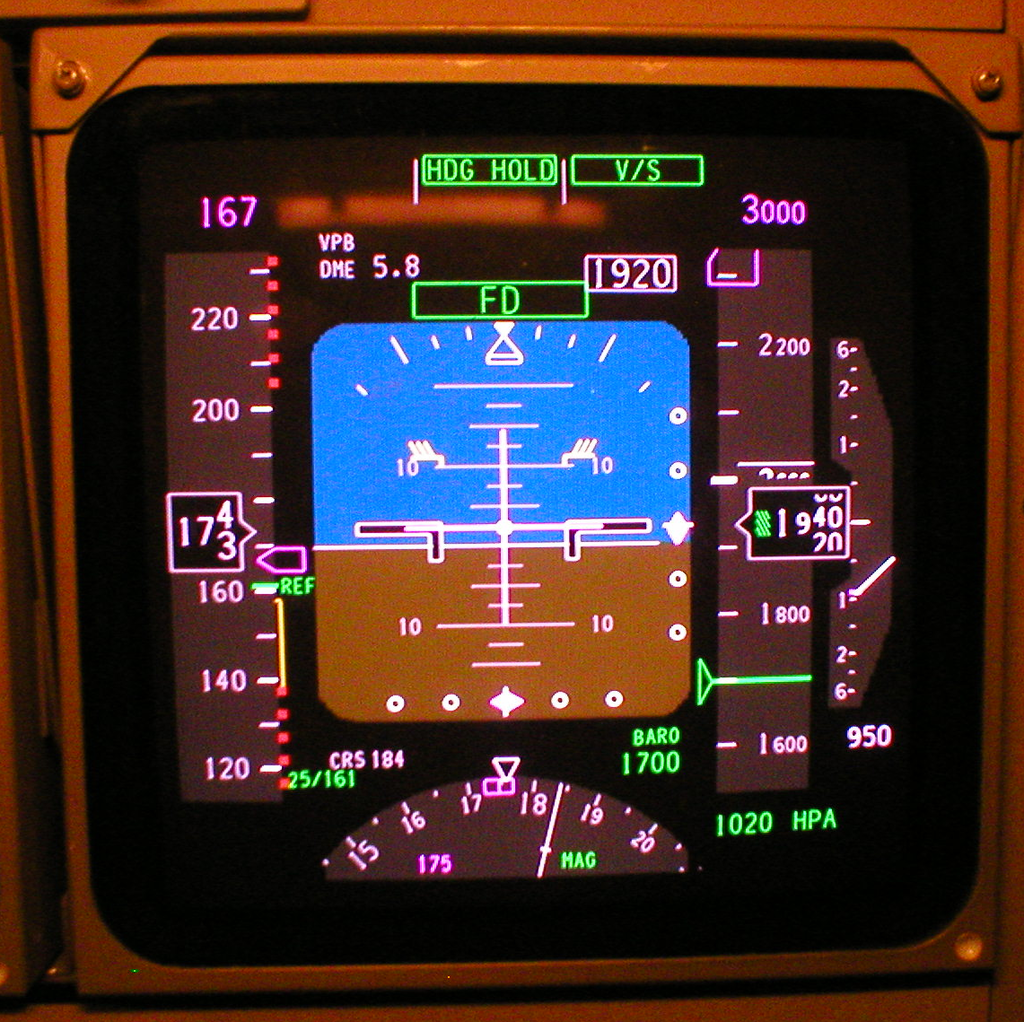
\includegraphics[width=3cm]{imagenes/1.4.pantalla.electronica/Primary_Flight_Display,_Boeing_747-400.png}\\
 

    \end{frame}      
    
\begin{frame}{Presentaci\'on en Pantalla Electr\'onica}

  \begin{block}{ MDF: MultiFunction Display o ND (Navigation Display)}

    Informaci\'on para navegaci\'on (VOR, DME, ILS)

    Informaci\'on clim\'atica de m\'ultiples sistemas (radar a bordo,
    sensores de detecci\'on de rel\'ampagos)

    Idem al PFD el MDF puede cambiar color, forma y dar alertas
    sonoras

    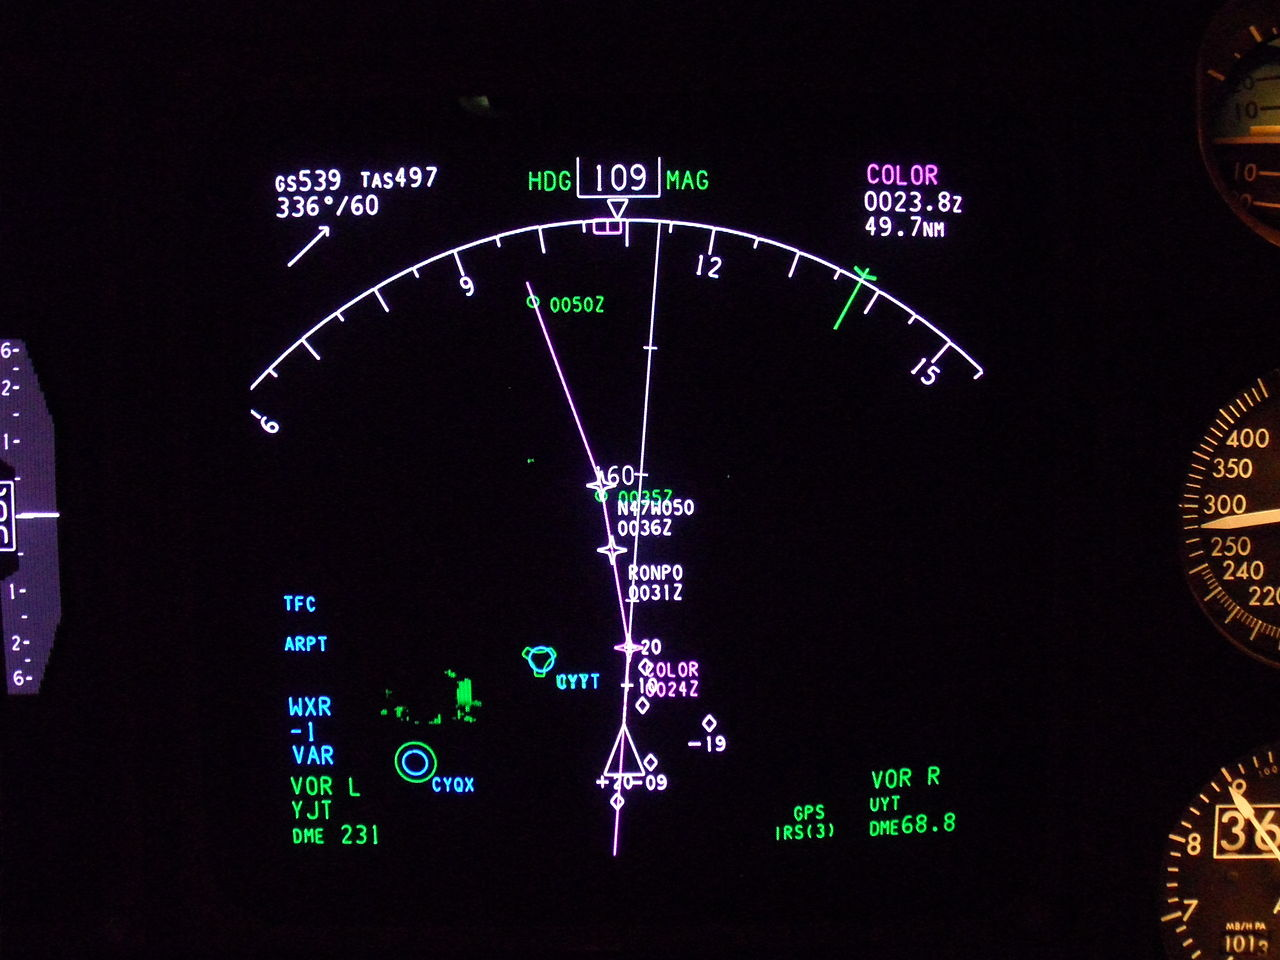
\includegraphics[width=6cm]{imagenes/1.4.pantalla.electronica/Navigation_Display_(ND)_on_Boeing_747-400.jpg}
  \end{block}
    \end{frame}      
    
\begin{frame}{Presentaci\'on en Pantalla Electr\'onica}

  \begin{block}{ ECAM : Electronic Centralized Aircraft Monitor
    (Airbus) \\
     EICAS : Electronic Centralized Aircraft Monitor (Boeing)}


    Monitorear los sistemas de la aeronave: p.e. combustible, sistemas
    el\'ectricos y del motor

    Usualmente dos (2) pantallas, una arriba de la otra

    La pantalla superior muestra sistemas motores, posici\'on flaps
    cantidad de combustible e informaci\'on de alerta

    La pantalla inferior muestra diversos par\'ametros de sistemas

    Brinda alarmas en caso de malfuncionamiento

    P.e. en caso de p\'erdida de presi\'on de aceite en un motor, el
    ECAM hace sonar una alerta, cambia la pantalla a una que muestra
    el sistema de aceite y se\~nala la baja presi\'on con una caja
    roja.

  \end{block}
    \end{frame}

\begin{frame}{Presentaci\'on en Pantalla Electr\'onica}
  \begin{tabular}{ccc}
	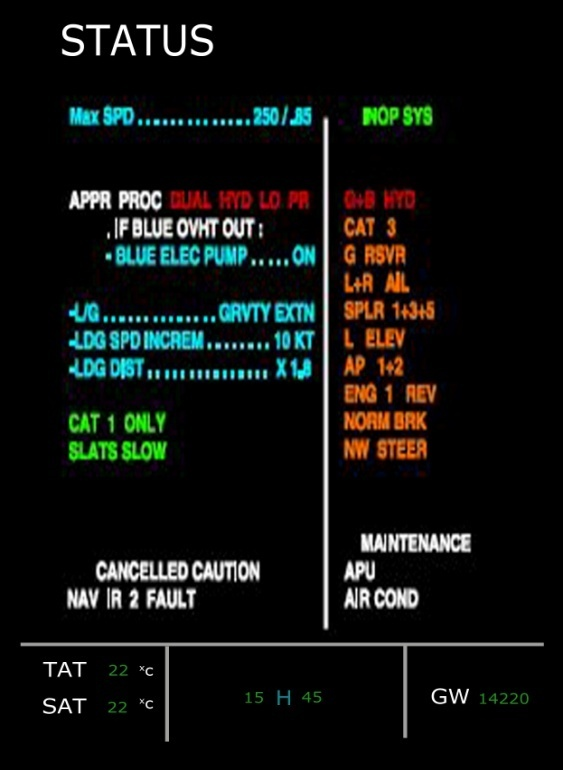
\includegraphics[width=4.5cm]{imagenes/1.4.pantalla.electronica/eicas_status.jpg}
	& \hspace{3mm} &
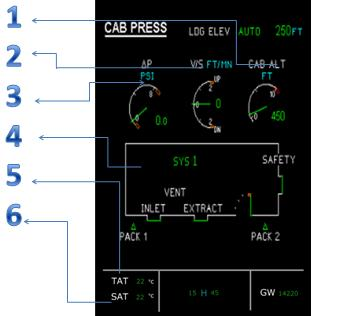
\includegraphics[width=6cm]{imagenes/1.4.pantalla.electronica/eicas_presion_cabina.jpg}
	\\
   	EICAS status & 
	& EICAS presi\'on cabina.  
% \parbox{\linewidth}{\tiny 1. Cabin altitude (height),
% 2. Vertical Speed (height/min),
% 3. Pressure,
% 4. Cabin,
% 5. True air temperature}
	\\
\end{tabular}

\end{frame}


\begin{frame}{Presentaci\'on en Pantalla Electr\'onica}
  \begin{center}
    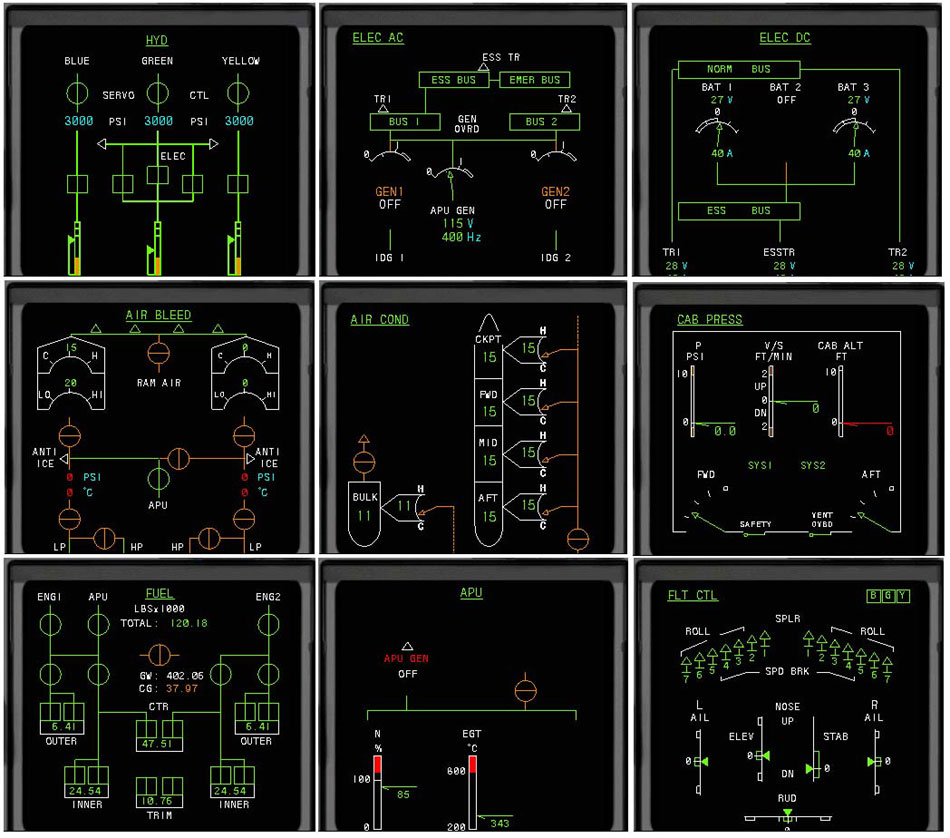
\includegraphics[width=0.65\textwidth]{imagenes/1.4.pantalla.electronica/ecam_airbus.jpg}

    \vspace{3mm}

    ECAM presentaci\'on
  \end{center}
\end{frame}

\begin{frame}{Presentaci\'on en Pantalla Electr\'onica}

  \begin{block} { FMS: Flight Management System}

    Instrumentos para mantener el plan de vuelo (flight plan) permite
    a los pilotos modificarlo en vuelo

    Dada la posici\'on y el plan de vuelo, el FMS se encarga de guiar
    el avi\'on a lo largo del mismo, gestiona los diversos factores
    que afectan al vuelo del avi\'on, tanto la ruta que tiene que
    seguir, como los niveles \'optimos a los cuales volar para reducir
    el consumo y hacer un vuelo m\'as eficiente.


    Usualmente se presenta como una pantalla peque\~na y un teclado

    El FMS se compone principalmente del CDU (control display unit) y
    el FMC (Flight Management Computer)
  \end{block}


% {\bf Autopiloto (AP)}

% 	Computadora que permite que una aeronave se vuele a s\'i misma.

% 	Se utiliza habitualmente en vuelos de larga duraci\'on

% 	El piloto se encuentra presente siempre para monitorear
% 	y chequear que el vuelo se desarrolle seg\'un el plan


% \end{itemize}

\end{frame}

\begin{frame}{Presentaci\'on en Pantalla Electr\'onica}


El piloto introduce los datos al FMC a trav\'es de la CDU que no es m\'as que un teclado y una pantalla que sirve para la comunicaci\'on entre el piloto y el FMC. A trav\'es de la CDU el piloto programa la ruta del vuelo, las SID (Standard Instrument Departures) y las STAR (Standard Terminal Arrival), as\'i como los puntos en las rutas donde el avi\'on debe ascender a niveles \'optimos seg\'un disminuye el peso del avi\'on.

    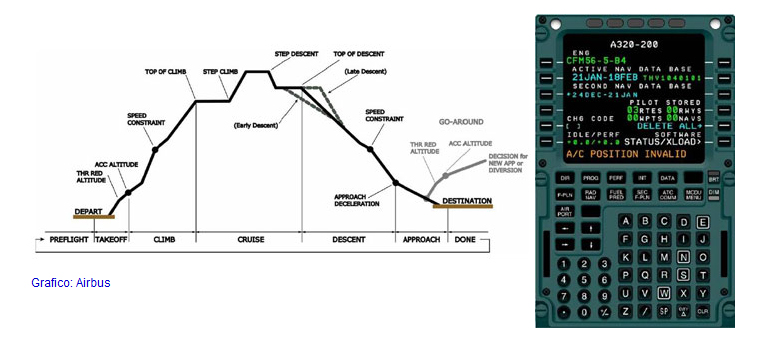
\includegraphics[width=0.9\textwidth]{imagenes/1.4.pantalla.electronica/fms_plan_vuelo.jpg}
  \end{frame}
  

\begin{frame}{Presentaci\'on en Pantalla Electr\'onica}
{\small
El FMC adem\'as adquiere datos de muchos de los sistemas del avi\'on. Para empezar recibe informaci\'on de los inerciales, y de los GPS para triangular la posici\'on del avi\'on y tener una posici\'on a\'un m\'as exacta de donde se encuentra el avi\'on.

El FMS tiene principalmente dos bases de datos. Una base de datos de navegaci\'on, donde est\'an almacenadas las rutas, aerov\'ias, SID, STARS, as\'i como las frecuencias de las radio ayudas a la navegaci\'on que va a sintonizar autom\'aticamente a lo largo de la ruta. Esta base de datos se renueva cada 28 d\'ias para poder estar actualizada cuando se producen cambios en los espacios a\'ereos o se modifican procedimientos de aproximaci\'on. El FMC es capaz de guardar dos bases de datos de navegaci\'on.

La otra base de datos es de performance del avi\'on. Esta base de datos contiene informaci\'on de los niveles \'optimos de vuelo dependiendo del peso del avi\'on. Los consumos que tiene el avi\'on para cada peso y nivel de vuelo. Las predicciones de ascenso y descenso del avi\'on.

Como el avi\'on va envejeciendo a lo largo de su vida y disminuyendo sus performance, el FMS admite un valor de degradaci\'on de las performance que se introduce en la p\'agina principal del CDU para que de unas previsiones de combustibles m\'as reales seg\'un el avi\'on se va haciendo ``mayor''
}
\end{frame}


\begin{frame}{Presentaci\'on en Pantalla Electr\'onica}

{\small
Con el tiempo el FMS ha ido mejorando y abarcando nuevas posibilidades. As\'i Airbus cambia el nombre al CDU y le ha pasado a llamar MCDU (Multi Control Display Unit). Ahora no solamente se puede acceder al FMC a trav\'es del teclado de la CDU si no a una infinidad de nuevos servicios.

Mediante el MCDU se accede al ATSU, AIDS, CFDS y al FMS comentado hasta ahora y llamado por Airbus FMGS (Flight Management Guidance System).

    El ATSU (Air Traffic Services Unit) es el acceso al Acars o sistema de comunicaciones tanto con la compa\~n\'ia como con el control a\'ereo. A trav\'es de esta opci\'on se recibe desde la hoja de carga, cualquier mensaje escrito que envie la compa\~n\'ia, hasta la autorizaci\'on para ingresar a otro pa\'is.

    El CFDS (Centralised Fault Display System) es usado principalmente por el personal de mantenimiento. En el est\'an los reportes de mantenimiento del vuelo, y las aver\'ias que haya tenido el avi\'on, por muy peque\~nas o temporales que hayan sido (aunque haya sido un fallo temporal de cualquier fusible por menos de 1 sg se queda registrado).

    El AIDS (Aircraft Integrated Data System) es otra herramienta que maneja mantenimiento, sirve para  interrogar y realizar TEST a cualquier sistema del avi\'on para conocer en qu\'e estado de operatividad se encuentra.

}
\end{frame}

\begin{frame}{Presentaci\'on en Pantalla Electr\'onica}

    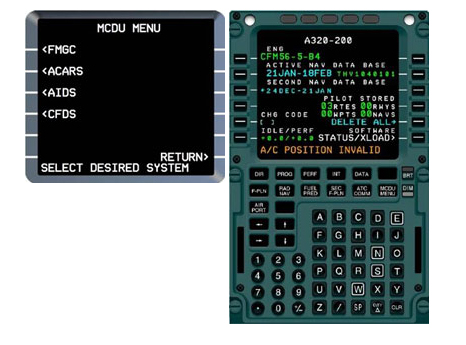
\includegraphics[width=0.9\textwidth]{imagenes/1.4.pantalla.electronica/mcdu.jpg}

\end{frame}


% %-------------Bibliografia
% \begin{frame}{Bibliograf\'ia}
%   \bibliographystyle{apalike} 
%   \bibliography{ventilacion}
% \end{frame}


\end{document}
